\documentclass[12pt]{article}
\usepackage{amsmath,amssymb}
\usepackage{newtxtext}
\usepackage[libertine]{newtxmath}
\usepackage{graphicx}
\usepackage{CJKutf8}
%%%%%%%%%%%%%%%%%%%%%%%%%%%%%%%%%%%%%%%%%%%%%%%%%%%%%%%%%%%%%%%%%%%%%%
%                        page size
\usepackage{geometry}
\geometry{left=25mm,right=25mm,top=20mm,bottom=30mm}
%%%%%%%%%%%%%%%%%%%%%%%%%%%%%%%%%%%%%%%%%%%%%%%%%%%%%%%%%%%%%%%%%%%%%%
%                        figure path
\graphicspath{{./fig/}}
%%%%%%%%%%%%%%%%%%%%%%%%%%%%%%%%%%%%%%%%%%%%%%%%%%%%%%%%%%%%%%%%%%%%%%
%                          often used macro

\newcommand{\Zb}{\mathbb{Z}}
\newcommand{\Rb}{\mathbb{R}}
\newcommand{\Cb}{\mathbb{C}}
\newcommand{\del}{\partial}
\newcommand{\SU}{\rm SU}
\newcommand{\SO}{\rm SO}
\newcommand{\Sp}{\rm Sp}
\newcommand{\g}{\mathfrac{g}}
\newcommand{\hc}{h^{\vee}}
\newcommand{\alc}{\alpha^{\vee}}
\newcommand{\ac}{a^{\vee}}
\newcommand{\dotrad}{0.2}
\DeclareMathOperator*{\Tr}{{\rm Tr}}

\newcommand{\extroot}[1]{{\color{green}\psset{linecolor=green} #1}}


%%%%%%%%%%%%%%%%%%%%%%%%%%%%%%%%%%%%%%%%%%%%%%%%%%%%%%%%%%%%%%%%%%%%%%
%\pagestyle{headings}
\begin{document}
\section*{Simple Lie algebra}
$\circ$: long root, $\bullet$: short root, $(j;a_j;a^{\vee}_j)$:
 (label;mark;comark), green line: $-\theta$,    $\theta$; highest root,
$W$:Weyl group, $P$: weight lattice,
$Q$ : root lattice, $Q^{\vee}$ : coroot lattice
$[\lambda_1,\dots,\lambda_r]$: Dynkin label.

Definitions and relations
\begin{align*}
 &\alc_j:=\frac{2}{|\alpha_j|^2}\alpha_j,
 &A_{ij}:=(\alpha_{i}|\alc_j),\\
 &\theta=\sum_{j=1}^{r}a_{j}\alpha_j=\sum_{j=1}^{r}\ac_j\alc_j,
 &\ac_{j}=\frac{|\alpha_j|^2}{2}a_{j},\\
 &h:=\sum_{j}a_j+1=\frac{|\Delta|}{r},
 &\hc:=\sum_{j}\ac_j+1,\\
 &(\omega_i| \alc_j)=\delta_{ij},
 &\alpha_i=\sum_{j=1}^{r} A_{ij}\omega_j,\\
 &\omega_i=\sum_{j=1}^{r} (A^{-1})_{ij}\alpha_j,
 &\rho:=\sum_{j=1}^{r}\omega_j=\frac12\sum_{\alpha\in\Delta_+}\alpha,\\
 &\dim \lambda =
      \prod_{\alpha\in\Delta_{+}}\frac{(\lambda+\rho|\alpha)}{(\rho|\alpha)},
 &|\rho|^2= \frac{\hc}{12}\dim G,
\end{align*}

\begin{thebibliography}{99}
  %\cite{DiFrancesco:1997nk}
\bibitem{DiFrancesco:1997nk}
P.~Di Francesco, P.~Mathieu and D.~Senechal,
``Conformal Field Theory,''
doi:10.1007/978-1-4612-2256-9
%%CITATION = doi:10.1007/978-1-4612-2256-9;%%
%110 citations counted in INSPIRE as of 27 Dec 2017
\bibitem{Sato}
\begin{CJK}{UTF8}{ipxm}佐藤光, ``群と物理,''丸善出版\end{CJK}
\end{thebibliography}
\newpage
%%%%%%%%%%%%%%%%%%%%%%%%%%%%%%%%%%%%%%%%%%%%%%%%%%%%%%%%%%%%%%%%%%%%%%%%
%
\subsection*{$A_r,\qquad r\ge 1,\qquad (\SU(r+1))$}
\parbox{8cm}{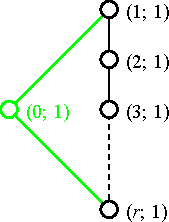
\includegraphics{lie_A.pdf}}
$
\begin{array}{l}
 \dim = r^2+2r, \\
 h=\hc= r+1,\\
 |W|=(r+1)!,\\
 \theta=[1,0,\dots,0,1],\\
 P/Q=\Zb_{r+1},\\
 \text{exponents}={\{1,2,\dots,r\}}
\end{array}
$

Cartan matrix:
\[A=\left(
\begin{array}{cccccc}
 2 & -1& 0 &\cdots & 0 & 0 \\
 -1& 2 & -1 &\cdots & 0 & 0 \\
 0 & -1 & 2 &\cdots & 0 & 0 \\
  \vdots&\vdots &\vdots &\ddots &\vdots &\vdots \\
 0&0 &0 &\cdots & 2& -1\\
 0&0 &0 &\cdots & -1& 2
\end{array}
\right)
\]
\[
A^{-1}=\frac{1}{r+1}
\left(
\begin{array}{cccccc}
 r & r-1& r-2 &\cdots & 2 & 1 \\
 r-1& 2(r-1) & 2(r-2) &\cdots & 4 & 2 \\
 r-2& 2(r-2) & 3(r-2) &\cdots & 6 & 3 \\
  \vdots&\vdots &\vdots &\ddots &\vdots &\vdots \\
 2&4 &6 &\cdots & 2(r-1)& r-1\\
 1&2 &3 &\cdots & r-1& r
\end{array}
\right)
\]

Quadratic form matrix: $A^{-1}$

Realization with orthonormal basis $e_j,\quad j=1,\dots,r+1$
\[
 \alpha_{j}=e_j-e_{j+1},\qquad j=1,2,\dots,r
\]
\[
 \Delta_{+}=\{e_i-e_j\ |\ i,j=1,\dots,r+1,\qquad i<j\}
\]

\newpage
%%%%%%%%%%%%%%%%%%%%%%%%%         B      %%%%%%%%%%%%%%%%%%%%%%%%%%%%%%%%%%%%
%
\subsection*{$B_r,\qquad r\ge 2,\qquad (\SO(2r+1))$}
\parbox{8cm}{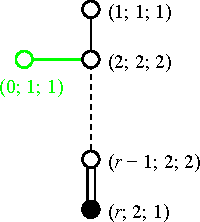
\includegraphics{lie_B.pdf}}
$
\begin{array}{l}
 \dim = 2r^2+r, \\
  h= 2 r,\\
 \hc= 2 r-1,\\
 |W|=2^r r!,\\
 \theta=[0,1,0,\dots,0,0],\\
 P/Q=\Zb_2,\\
 \text{exponents}={\{1,3,\dots,2r-1\}}
\end{array}
$

Cartan matrix:
\[
A=\left(
\begin{array}{cccccc}
 2 & -1& 0 &\cdots & 0 & 0 \\
 -1& 2 & -1 &\cdots & 0 & 0 \\
 0 & -1 & 2 &\cdots & 0 & 0 \\
  \vdots&\vdots &\vdots &\ddots &\vdots &\vdots \\
 0&0 &0 &\cdots & 2& -2\\
 0&0 &0 &\cdots & -1& 2
\end{array}
\right),\quad
A^{-1}=\frac{1}{2}
\left(
\begin{array}{cccccc}
 2& 2& 2 &\cdots & 2 & 2 \\
 2& 4 & 4 &\cdots & 4 & 4 \\
 2& 4 & 6 &\cdots & 6 & 6 \\
  \vdots&\vdots &\vdots &\ddots &\vdots &\vdots \\
 2&4 &6 &\cdots & 2(r-1)& 2(r-1)\\
 1&2 &3 &\cdots & r-1& r/2
\end{array}
\right)
\]

Quadratic form matrix:
\[\frac{1}{2}
\left(
\begin{array}{cccccc}
 2& 2& 2 &\cdots & 2 & 1 \\
 2& 4 & 4 &\cdots & 4 & 2 \\
 2& 4 & 6 &\cdots & 6 & 3 \\
  \vdots&\vdots &\vdots &\ddots &\vdots &\vdots \\
 2&4 &6 &\cdots & 2(r-1)& r-1\\
 1&2 &3 &\cdots & r-1& r
\end{array}
\right)
\]

Realization with orthonormal basis $e_j,\quad j=1,\dots,r$

\begin{align*}
  &\alpha_{j}=e_j-e_{j+1},\qquad j=1,2,\dots,r-1,\\
  &\alpha_{r}=e_r
\end{align*}

\begin{align*}
 \Delta_{+}=&\{e_i \pm e_j\ |\ i,j=1,\dots,r+1,\qquad i<j\} \\
      &\cap
       \{e_{i}\ |\ i=1,\dots,r\}
\end{align*}

\newpage
%%%%%%%%%%%%%%%%%%%%%%%%%        C      %%%%%%%%%%%%%%%%%%%%%%%%%%%%%%%%%%%%
%
\subsection*{$C_r,\qquad r\ge 2,\qquad (\Sp(r))$}
\parbox{8cm}{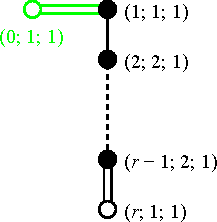
\includegraphics{lie_C.pdf}}
$
\begin{array}{l}
 \dim = 2r^2+r, \\
  h= 2r,\\
 \hc= r+1,\\
 |W|=2^r r!,\\
 \theta=[2,0,\dots,0],\\
 P/Q=\Zb_2,\\
 \text{exponents}={\{1,3,\dots,2r-1\}}
\end{array}
$

Cartan matrix:
\[
A=\left(
\begin{array}{cccccc}
 2 & -1& 0 &\cdots & 0 & 0 \\
 -1& 2 & -1 &\cdots & 0 & 0 \\
 0 & -1 & 2 &\cdots & 0 & 0 \\
  \vdots&\vdots &\vdots &\ddots &\vdots &\vdots \\
 0&0 &0 &\cdots & 2& -1\\
 0&0 &0 &\cdots & -2& 2
\end{array}
\right)
,\quad
A^{-1}=\frac{1}{2}
\left(
\begin{array}{cccccc}
 2& 2& 2 &\cdots & 2 & 1 \\
 2& 4 & 4 &\cdots & 4 & 2 \\
 2& 4 & 6 &\cdots & 6 & 3 \\
  \vdots&\vdots &\vdots &\ddots &\vdots &\vdots \\
 2&4 &6 &\cdots & 2(r-1)& r-1\\
 2&4 &6 &\cdots & 2(r-1)& r
\end{array}
\right)
\]

Quadratic form matrix:
\[\frac{1}{2}
\left(
\begin{array}{cccccc}
 1& 1& 1 &\cdots & 1 & 1 \\
 1& 2 & 2 &\cdots & 2 & 2 \\
 1& 2 & 3 &\cdots & 3 & 3 \\
  \vdots&\vdots &\vdots &\ddots &\vdots &\vdots \\
 1&2 &3 &\cdots & r-1& r-1\\
 1&2 &3 &\cdots & r-1& r
\end{array}
\right)
\]

Realization with orthonormal basis $e_j,\quad j=1,\dots,r$

\begin{align*}
  &\alpha_{j}=(e_j-e_{j+1})/\sqrt{2},\qquad j=1,2,\dots,r-1,\\
  &\alpha_{r}=\sqrt{2} e_r
\end{align*}

\begin{align*}
 \Delta_{+}=&\{(e_i \pm e_j)/\sqrt{2}\ |\ i,j=1,\dots,r+1,\qquad i<j\} \\
      &\cap
       \{ \sqrt{2}e_{i}\ |\ i=1,\dots,r\}
\end{align*}
\newpage

%%%%%%%%%%%%%%%%%%%%%%%%%         D      %%%%%%%%%%%%%%%%%%%%%%%%%%%%%%%%%%%%
%
\subsection*{$D_r,\qquad r\ge 4,\qquad (\SO(2r))$}
\parbox{8cm}{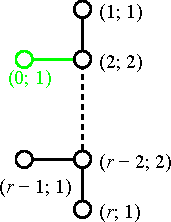
\includegraphics{lie_D.pdf}}
$
\begin{array}{l}
 \dim = 2r^2-r, \\
  h=\hc= 2 r-2,\\
 |W|=2^{r-1} r!,\\
 \theta=[0,1,0,\dots,0],\\
 P/Q=\Zb_4\ (r:\text{odd}), \\
  \qquad\    =\Zb_2 \times \Zb_2\ (r:\text{even}),\\
 \text{exponents}={\{1,3,\dots,2r-3,r-1\}}
\end{array}
$

Cartan matrix:
\[
A=\left(
\begin{array}{ccccccc}
 2 & -1& 0 &\cdots & 0 & 0  &0 \\
 -1& 2 & -1 &\cdots & 0 & 0 &0 \\
 0 & -1 & 2 &\cdots & 0 & 0 &0 \\
  \vdots&\vdots &\vdots &\ddots &\vdots &\vdots&\vdots \\
 0&0 &0 &\cdots & 2& -1 & -1\\
 0&0 &0 &\cdots & -1& 2 &  0 \\
 0&0 &0 &\cdots & -1 & 0 & 2\\
\end{array}
\right)\]
\[
A^{-1}=\frac{1}{2}
\left(
\begin{array}{ccccccc}
 2& 2& 2 &\cdots & 2 & 1 & 1 \\
 2& 4 & 4 &\cdots & 4 & 2 & 2 \\
 2& 4 & 6 &\cdots & 6 & 3 & 3 \\
  \vdots&\vdots &\vdots &\ddots &\vdots &\vdots &\vdots \\
 2&4 &6 &\cdots & 2(r-2)& r-2 & r-2\\
 1&2 &3 &\cdots & r-2  & r/2 & (r-2)/2\\
 1&2 &3 &\cdots & r-2  & (r-2)/2 & r/2\\
\end{array}
\right)
\]

Quadratic form matrix: $A^{-1}$

Realization with orthonormal basis $e_j,\quad j=1,\dots,r$

\begin{align*}
  &\alpha_{j}=e_j-e_{j+1},\qquad j=1,2,\dots,r-1,\\
  &\alpha_{r}=e_{r-1}+e_{r}
\end{align*}

\begin{align*}
 \Delta_{+}=&\{e_i \pm e_j\ |\ i,j=1,\dots,r+1,\qquad i<j\}
\end{align*}
\newpage
%%%%%%%%%%%%%%%%%%%%%%%%%         E_6      %%%%%%%%%%%%%%%%%%%%%%%%%%%%%%%%%%%%
%
\subsection*{$E_6$}
\parbox{8cm}{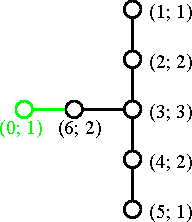
\includegraphics{lie_E6.pdf}}
$
\begin{array}{l}
 \dim = 78, \\
  h=\hc= 12,\\
 |W|= 51840,\\
 \theta=[0,0,0,0,0,1],\\
 P/Q=\Zb_3 \\
 \text{exponents}={\{1,4,5,7,8,11\}}
\end{array}
$

Cartan matrix:
\[
A=\left(
\begin{array}{cccccc}
 2 &-1& 0& 0& 0&0   \\
 -1& 2&-1& 0& 0& 0 \\
 0 &-1& 2&-1& 0& -1 \\
 0 &0 &-1& 2&-1&  0\\
 0 &0 &0 &-1& 2&  0 \\
 0 &0 &-1 & 0& 0& 2\\
\end{array}
\right)\]
\[
A^{-1}=
\frac{1}{3}\left(
\begin{array}{cccccc}
  4& 5& 6& 4& 2& 3 \\
  5&10&12& 8& 4& 6 \\
  6&12&18&12& 6& 9 \\
  4& 8&12&10& 5& 6 \\
  2& 4& 6& 5& 4& 3 \\
  3& 6& 9& 6& 3& 6 \\
\end{array}
\right)
\]

Quadratic form matrix: $A^{-1}$

%Realization with orthonormal basis $e_j,\quad j=1,\dots,6$
%
%\begin{align*}
%  &\alpha_{j}=e_j-e_{j+1},\qquad j=1,2,\dots,r-1,\\
%  &\alpha_{r}=e_{r-1}+e_{r}
%\end{align*}
%
%\begin{align*}
% \Delta_{+}=&\{e_i \pm e_j\ |\ i,j=1,\dots,r+1,\qquad i<j\}
%\end{align*}
\newpage
%%%%%%%%%%%%%%%%%%%%%%%%%         E_7      %%%%%%%%%%%%%%%%%%%%%%%%%%%%%%%%%%%%
%
\subsection*{$E_7$}
\parbox{8cm}{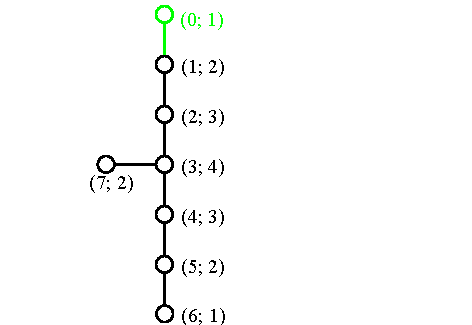
\includegraphics{lie_E7.pdf}}
$
\begin{array}{l}
 \dim = 133, \\
  h=\hc= 18,\\
 |W|= 2903040,\\
 \theta=[1,0,0,0,0,0,0],\\
 P/Q=\Zb_2 \\
 \text{exponents}={\{1,5,7,9,11,13,17\}}
\end{array}
$

Cartan matrix:
\[
A=\left(
\begin{array}{ccccccc}
 2 &-1& 0& 0& 0 & 0 &0   \\
 -1& 2&-1& 0& 0 & 0 & 0 \\
 0 &-1& 2&-1& 0 & 0 & -1 \\
 0 &0 &-1& 2&-1 & 0 & 0\\
 0 &0 &0 &-1& 2 &-1 & 0 \\
 0 &0 & 0 & 0&-1& 2 & 0\\
 0 &0 &-1 & 0& 0& 0 & 2\\
\end{array}
\right)\]
\[
A^{-1}=
\frac{1}{2}\left(
\begin{array}{ccccccc}
  4& 6& 8& 6& 4& 2& 4 \\
  6&12&16&12& 8& 4& 8 \\
  8&16&24&18&12& 6& 12 \\
  6&12&18&15&10& 5& 9 \\
  4& 8&12&10& 8& 4& 6 \\
  2& 4& 6& 5& 4& 3& 3 \\
  4& 8&12& 9& 6& 3& 7 \\
\end{array}
\right)
\]

Quadratic form matrix: $A^{-1}$

%Realization with orthonormal basis $e_j,\quad j=1,\dots,6$
%
%\begin{align*}
%  &\alpha_{j}=e_j-e_{j+1},\qquad j=1,2,\dots,r-1,\\
%  &\alpha_{r}=e_{r-1}+e_{r}
%\end{align*}
%
%\begin{align*}
% \Delta_{+}=&\{e_i \pm e_j\ |\ i,j=1,\dots,r+1,\qquad i<j\}
%\end{align*}
\newpage
%%%%%%%%%%%%%%%%%%%%%%%%%         E_8      %%%%%%%%%%%%%%%%%%%%%%%%%%%%%%%%%%%%
%
\subsection*{$E_8$}
\parbox{8cm}{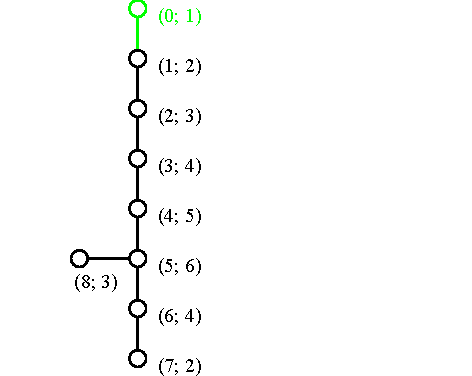
\includegraphics{lie_E8.pdf}}
$
\begin{array}{l}
 \dim = 248, \\
  h=\hc= 30,\\
 |W|= 696729600,\\
 \theta=[1,0,0,0,0,0,0,0],\\
 P/Q=\{1\} \\
 \text{exponents}={\{1,7,11,13,17,19,23,29\}}
\end{array}
$

Cartan matrix:
\[
A=\left(
\begin{array}{cccccccc}
 2 &-1& 0& 0& 0& 0 & 0 &0   \\
 -1& 2&-1& 0& 0& 0 & 0 &0   \\
 0 &-1& 2&-1& 0& 0 & 0 & 0 \\
 0 &0 &-1& 2&-1& 0 & 0 & 0 \\
 0 &0 &0 &-1& 2&-1 & 0 & -1\\
 0 &0 &0 &0 &-1& 2 &-1 & 0 \\
 0 &0 &0 & 0 & 0&-1& 2 & 0\\
 0 &0 &0 & 0 &-1& 0& 0 & 2\\
\end{array}
\right)\]
\[
A^{-1}=
\left(
\begin{array}{cccccccc}
   2& 3& 4& 5& 6& 4& 2& 3\\
   3& 6& 8&10&12& 8& 4& 6\\
   4& 8&12&15&18&12& 6& 9\\
   5&10&15&20&24&16& 8&12\\
   6&12&18&24&30&20&10&15\\
   4& 8&12&16&20&14& 7&10\\
   2& 4& 6& 8&10& 7& 4& 5\\
   3& 6& 9&12&15&10& 5& 8\\
\end{array}
\right)
\]

Quadratic form matrix: $A^{-1}$

%Realization with orthonormal basis $e_j,\quad j=1,\dots,6$
%
%\begin{align*}
%  &\alpha_{j}=e_j-e_{j+1},\qquad j=1,2,\dots,r-1,\\
%  &\alpha_{r}=e_{r-1}+e_{r}
%\end{align*}
%
%\begin{align*}
% \Delta_{+}=&\{e_i \pm e_j\ |\ i,j=1,\dots,r+1,\qquad i<j\}
%\end{align*}
\newpage
%%%%%%%%%%%%%%%%%%%%%%%%%         F_4    %%%%%%%%%%%%%%%%%%%%%%%%%%%%%%%%%%%%
%
\subsection*{$F_4$}
\parbox{8cm}{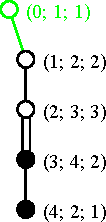
\includegraphics{lie_F4.pdf}}
$
\begin{array}{l}
 \dim = 52, \\
  h= 12,\\
 \hc= 9,\\
 |W|=1152,\\
 \theta=[1,0,0,0],\\
 P/Q=\{0\},\\
 \text{exponents}={\{1,5,7,11\}}
\end{array}
$

Cartan matrix:
\[
A=\left(
\begin{array}{cccc}
 2& -1& 0& 0\\
 -1& 2& -2&0 \\
 0 &-1 &2 &-1 \\
 0 &0  &-1 &2 \\
\end{array}
\right),\quad
A^{-1}=\left(
\begin{array}{cccc}
 2& 3 & 4& 2\\
 3 & 6&  8&4 \\
 2 & 4 &6 & 3 \\
 1 &2  & 3 &2 \\
\end{array}
\right)
\]

Quadratic form matrix:
\[
\left(
\begin{array}{cccc}
 2& 3 & 2& 1\\
 3 & 6& 4&2 \\
 2 & 4 & 3 & \frac32 \\
 1 &2  & \frac32 &1 \\
\end{array}
\right)
\]

Realization with orthonormal basis $e_j,\quad j=1,2,3,4$

\begin{align*}
  &\alpha_1=e_2-e_3,\qquad
  \alpha_2=e_3-e_4,\qquad
  \alpha_3=e_4,\qquad
  \alpha_4=\frac12(e_1-e_2-e_3-e_4).
\end{align*}

\begin{align*}
 \Delta_{+}=&\{(e_i \pm e_j)\ |\ i,j=1,2,3,4,\qquad i<j\} \\
      &\cap
       \{ e_{i}\ |\ i=1,2,3,4\}\\
      &\cap
       \{ (e_{1}\pm e_2 \pm e_3 \pm e_4)/2\}
\end{align*}
\newpage

%%%%%%%%%%%%%%%%%%%%%%%%%         G_2      %%%%%%%%%%%%%%%%%%%%%%%%%%%%%%%%%%%%
%
\subsection*{$G_2$}
\parbox{8cm}{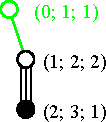
\includegraphics{lie_G2.pdf}}
$
\begin{array}{l}
 \dim = 14, \\
  h= 6,\\
 \hc= 4,\\
 |W|=12,\\
 \theta=[1,0],\\
 P/Q=\{0\},\\
 \text{exponents}={\{1,5\}}
\end{array}
$

Cartan matrix:
\[
A=\left(
\begin{array}{cc}
 2 & -3 \\
 -1& 2
\end{array}
\right),\quad
A^{-1}=\left(
\begin{array}{cc}
 2 & 3 \\
 1& 2
\end{array}
\right)
\]

Quadratic form matrix:
\[\frac{1}{3}
\left(
\begin{array}{cc}
 6& 3 \\
 3& 2
\end{array}
\right)
\]

Realization with orthonormal basis $e_j,\quad j=1,2,3$

\begin{align*}
  &\alpha_1=e_2-e_3,\qquad
  \alpha_2=\frac13(e_1-e_2+2e_3)
\end{align*}

\begin{align*}
 \Delta_{+}=\left\{e_2-e_3,\ \frac13(e_1-e_2+2e_3),\ \frac13(e_1+2e_2-e_3),\
   \frac13(2e_1+e_2+e_3),\ e_1+e_3,\ e_1+e_2
  \right\}
\end{align*}
\end{document}
